\chapter{Introduction}
\label{Chapter:Intro}



%%%%%%%%%%%%%%%%%%%%%%%%%%%%%%%%%%%%%%%%%%%%%%%%%%%%%%%%%
%                                                       %
%                   S E C T I O N                       %
%                                                       %
%%%%%%%%%%%%%%%%%%%%%%%%%%%%%%%%%%%%%%%%%%%%%%%%%%%%%%%%%
\section{Software Crisis}  \label{Intro:Crisis}

Software ``production'' is inherently different from manufacturing production. Every software project is unique. Despite tremendous research effort invested by the software engineering community for the past several decades to build reliable software efficiently and effectively, software development methods, as currently practiced, still remain largely an art. Software development is slow, expensive and error prone, often resulting in products with large number of defects which cause serious problems in usability, reliability and performance.

According to \textit{the Chaos Report} \cite{Standish:1994} published by the Standish group, companies in the United States spent more than \$250 billion each year on IT application development of approximately 175,000 projects. Only 16\% of these projects finished on schedule and within budget. Another 31\% were cancelled before completion, mainly due to quality problems, for losses of about \$81 billion. Approximately 53\% exceeded their original budgets by an average of 189\% for losses of about \$59 billion. Those projects that managed to final completion delivered an average of 42\% of the planned features. The direct cost of these failures and overruns were just the tip of the iceberg. The loss of indirect opportunity costs were not measured in the report, but could easily be trillions of dollars.

A report \cite{Peterson:1997} from the Software Engineering Institute (SEI) indicated that out of 542 software organizations participating in the CMM maturity assessment, 67\% of them were at CMM Level 1 (the lowest process maturity level), and 20\% were at CMM Level 2. The software process at CMM Level 1 is characterized as \textit{ad hoc} and sometimes \textit{chaotic}. Inputs to the process are ill-defined, and the transition from inputs to final software products is uncontrolled. The development process is so reactive that management control is impossible. The development process at CMM Level 2 is better, because earlier successes on projects with similar applications can potentially be repeated. However, there is still no visibility as to how software products are produced, and any disturbance to the development team or resources can easily cause project failure. In other words, 87\% of the software organizations in the survey were unable to control their development processes. Nor were they able to consistently develop software products on schedule and within budget. 

Uncontrollable and non-repeatable processes cause many problems for software development organizations. For example, it becomes hard to ensure software quality, hard to make reliable effort and schedule estimation, and impossible to allocate resources efficiently.



%%%%%%%%%%%%%%%%%%%%%%%%%%%%%%%%%%%%%%%%%%%%%%%%%%%%%%%%%
%                                                       %
%                   S E C T I O N                       %
%                                                       %
%%%%%%%%%%%%%%%%%%%%%%%%%%%%%%%%%%%%%%%%%%%%%%%%%%%%%%%%%
\section{Software Measurement, Process Improvement, and Predictions}  \label{Intro:Measurement}

It is conventional wisdom that ``\textit{you can neither predict nor control what you cannot measure} \cite{DeMarco:1982}.'' Consistent measurement is a key component in establishing a scientific basis for software engineering. Software metrics are capable of quantifying software products and their development processes in an objective way. They make aspects of processes and products more visible, and give us better understanding of the relationship between development activities and the attributes of software products they affect. As a result, various measurement programs have been developed to improve software organizations' development processes and their capability to produce software products in a controllable and repeatable manner. 

Effective measurement programs help software organizations understand their capabilities, so that they can develop achievable plans for producing and delivering software products. Furthermore, continual measurement can provide an effective foundation for managing process improvement activities. The end result is that software organizations have controllable and repeatable development processes, and possess the ability to make reliable predictions about their development activities.

Indeed, software measurement is always at the core of software process improvement and assessment programs, such as PSP \cite{Humphrey:1995, Humphrey:1996}, CMM \cite{Humphrey:1989, Paulk:1993, Humphrey:1995}, ISO 9001 \cite{ISO9001:1987}, SPICE \cite{ISO:1998, Eman:1998} and BOOTSTRAP \cite{Kuvaja:1994}. Industrial experiences \cite{Grady:1987} have demonstrated that so long as measurement programs are conscientiously followed, they can help software organizations achieve improved development processes, both in the short run and in the long run. Controllable and repeatable processes are essential for software organizations to make reliable predictions about their development activities, such as those in SLIM \cite{Putnam:1978, SLIM} and COCOMO \cite{Cocomo:1981, Cocomo:2000}.





%%%%%%%%%%%%%%%%%%%%%%%%%%%%%%%%%%%%%%%%%%%%%%%%%%%%%%%%%
%                                                       %
%                   S E C T I O N                       %
%                                                       %
%%%%%%%%%%%%%%%%%%%%%%%%%%%%%%%%%%%%%%%%%%%%%%%%%%%%%%%%%
\section{Problem Statement}  \label{Intro:Problem}


Despite the potential for software measurement in theory and positive experiences \cite{Grady:1987} in reality, effective application appears far from mainstream in practice. For example, a recent case study \cite{Kulik:2003} surveyed 630 software professionals. It divided software development organizations into two groups: ``best practice'' and ``all other.'' Only 27\% of the ``best practice'' organizations responded that reliance on metrics and measurements when making project-related decisions was \textit{very} or \textit{extremely} important, while this number is just 2\% for organizations in the ``all other'' category. 

Research has identified a variety of reasons for this discrepancy. They can be categorized into two major groups:
\begin{itemize}
  \setlength{\itemsep}{0pt}
  \setlength{\parskip}{0pt}
  \item The Metrics Collection Cost Problem
  \item The Metrics Decision-making Problem
\end{itemize}



\subsection{Metric Collection Cost Problem}

All measurement activities compete for resources. An important question that a software organization committing itself to measurement program must answer is whether the benefit from measurement outweighs the cost. Existing measurement programs tend to be very expensive. For example, the PSP uses manual metrics collection. It is not only tedious, but also susceptible to bias, error, omission, and delay. The adoption of tool-based metrics collection techniques, such as LEAP \cite{Moore:1999}, PSP Studio \cite{PspStudio:1997}, and Software Process Dashboard \cite{PspDashboard:2000}, does not completely solve these problems because of their chronic overhead that requires the user to constantly switch back and forth between doing work and telling the tool what work is being done \cite{Johnson:2001, Johnson:2003}. CMM requires that measurement be taken in all key process areas in order to determine the status of the activities. Quantitative measurement is mandatory in CMM Level 4 and 5. Humphrey himself admitted that:

\begin{quote}
\textit{``The greatest potential problem with the managed process is the cost of gathering data, and that there are an enormous number of potentially valuable measures of the software process, but such data are expensive to gather and to maintain.''} \cite{Humphrey:1988}
\end{quote}

Due to the high cost associated with metrics collection, it is a daunting task to apply measurement best practices to improve a software organization's development process in practice. 



	
\subsection{Metrics Decision-Making Problem}

The metrics decision-making problem refers to the problem of how to make project management and process improvement decisions based on information in the metrics. Traditional approaches use a ``historical project database'' as a baseline for comparison with metrics from the current project. They typically involve the following procedure: (1) collect a set of process and product metrics, such as size, effort, complexity, and defects, for a set of completed software projects, (2) generate a model to fit the collected metrics, (3) claim that the model can be used to predict characteristics of future projects. Project management and process improvement is based on the predictions made by the models. For example, one model might predict that a future project of size \textit{S} would require \textit{E} person-months of effort, another model might predict that a future implementation of a module with complexity \textit{C} would be prone to defects with density \textit{D}, and so forth.

This model-based process prediction technique is used in many forms, such as PSP (Section \ref{RelatedWork:PSP}) and COCOMO (Section \ref{RelatedWork:COCOMO}). The technique faces a number of limitations:

\begin{itemize}
	\item First, the predictive power of the model depends crucially on how well model calibration is performed. In order to use the model off-the-shelf, practitioners must confirm that the set of projects used to calibrate the model are ``comparable'' to the project they wish to predict. Otherwise, the model must be recalibrated using the data in the organization's historical project database to avoid the problem of comparing apples to oranges. Apart from the cost of accumulating the historical project database, recalibration involves replicating the model-building method within the practitioner's organization, with the risk that the applications, personnel, and resources may have already changed, and the context of the current project may differ from those in the historical project database. 

  \item Second, model-based process prediction assumes that a software organization's development process is predictable. However, according to the SEI survey \cite{Peterson:1997}, 67\% of the surveyed organizations were at the lowest CMM maturity level. By definition, the software processes at that level are \textit{ad hoc} and sometimes \textit{chaotic}, and they change as work changes. It is simply impossible to make predictions for these organizations. As a result, the majority of software development organizations are incapable of benefiting from model-based approches to improve their development processes.
  
  \item Lastly, most models available are built to compare a set of finished projects. This may be useful for initial project planning. But if you want to manage a project that is still being developed, most models are not designed with such in-process control in mind. In other words, how do you use metrics from completed projects to manage a project that is still in progress?  
  
\end{itemize}


The result is the dilemma we are facing today. Almost all software organizations are aware of the benefits of a mature development process and the value of measurement programs in achieving it, but few of them are capable of implementing a successful measurement program in practice. Many of the difficulties lie in one or both of the \textit{``metrics collection cost''} and \textit{``metrics decision-making''} problems.






%%%%%%%%%%%%%%%%%%%%%%%%%%%%%%%%%%%%%%%%%%%%%%%%%%%%%%%%%
%                                                       %
%                   S E C T I O N                       %
%                                                       %
%%%%%%%%%%%%%%%%%%%%%%%%%%%%%%%%%%%%%%%%%%%%%%%%%%%%%%%%%
\section{Proposed Solution - Software Project Telemetry}  \label{Intro:Solution}

In this thesis, I propose a novel approach to software measurement called \textit{``software project telemetry''}. 
It addresses the \textit{``metrics collection cost problem''} through highly automated measurement machinery: software sensors are written to collect metrics automatically and unobtrusively. 
It addresses the \textit{``metrics decision-making problem''} through a domain-specific language designed for the representation of telemetry trends for different aspects of software development process.

In contrast to model-based approaches, which involve the comparison of data from different projects, software project telemetry focuses on the comparison of data taken from the same project at different times. This within-project data comparison involves a much smaller time scale: typically with intervals of days or weeks. The idea is that comparison can be made more effectively between two different periods of the same project than between two different projects. It thus avoids many problems a model-based approach suffers from, such as spending the cost of accumulating a historical project database first and then constantly worrying about whether the current project is �comparable� to those in the database.
In software project telemetry, the metrics from the initial period of the project are used to establish a baseline and bootstrap the process. Project management and process improvement decisions are made by detecting changes in telemetry trends and comparing trends between two periods of the same project. In-process control for a project that is still being developed is made possible precisely because comparisons are made within the same project instead of across projects.







\subsection{Metrics Collection}
\label{Intro:Solution:MetricsCollection}

In software project telemetry, sensors collect metrics \textit{automatically} and \textit{unobtrusively}. Sensors are pieces of software that monitor some form of state in the project development environment. They collect both software \textit{process} and \textit{product} metrics.

Software process metrics are the metrics that assist in monitoring and controlling the way software is produced. Sensors collecting process metrics are typically implemented in the form of plug-ins, which are attached to software development tools in order to continuously monitor and record their activities in the background. Some examples are (1) a sensor for an IDE that monitors developer activities, such as code editing effort, compilation attempts and results, etc., or (2) a sensor for an integration build system that monitors the number of times the program failed to rebuild overnight. 

Software product metrics are the metrics that describes the properties of the software itself. Sensors collecting product metrics are typically implemented as analyzers for software artifacts. An example is an analyzer that parses program source code to compute size and complexity information.

There are many possibilities for sensors and the data that they collect. However, the key point is that sensors are designed to collect metrics automatically and unobtrusively. This way, sensors not only keep metrics collection cost low, but also enable developers to focus on their primary task -- developing software products instead of recording process and product metrics.





\subsection{Metrics Decision-making}
\label{Intro:Solution:MetricsAnalysis}

The metrics collected by sensors are time-stamped, and these time stamps are always significant in metrics analysis. Telemetry streams, charts, and reports capture high-level perspectives on software development, while the telemetry language facilitates the exploration of these perspectives in telemetry analyses. Telemetry analyses can be performed at different levels. 

\begin{figure}[p]
  \centering
  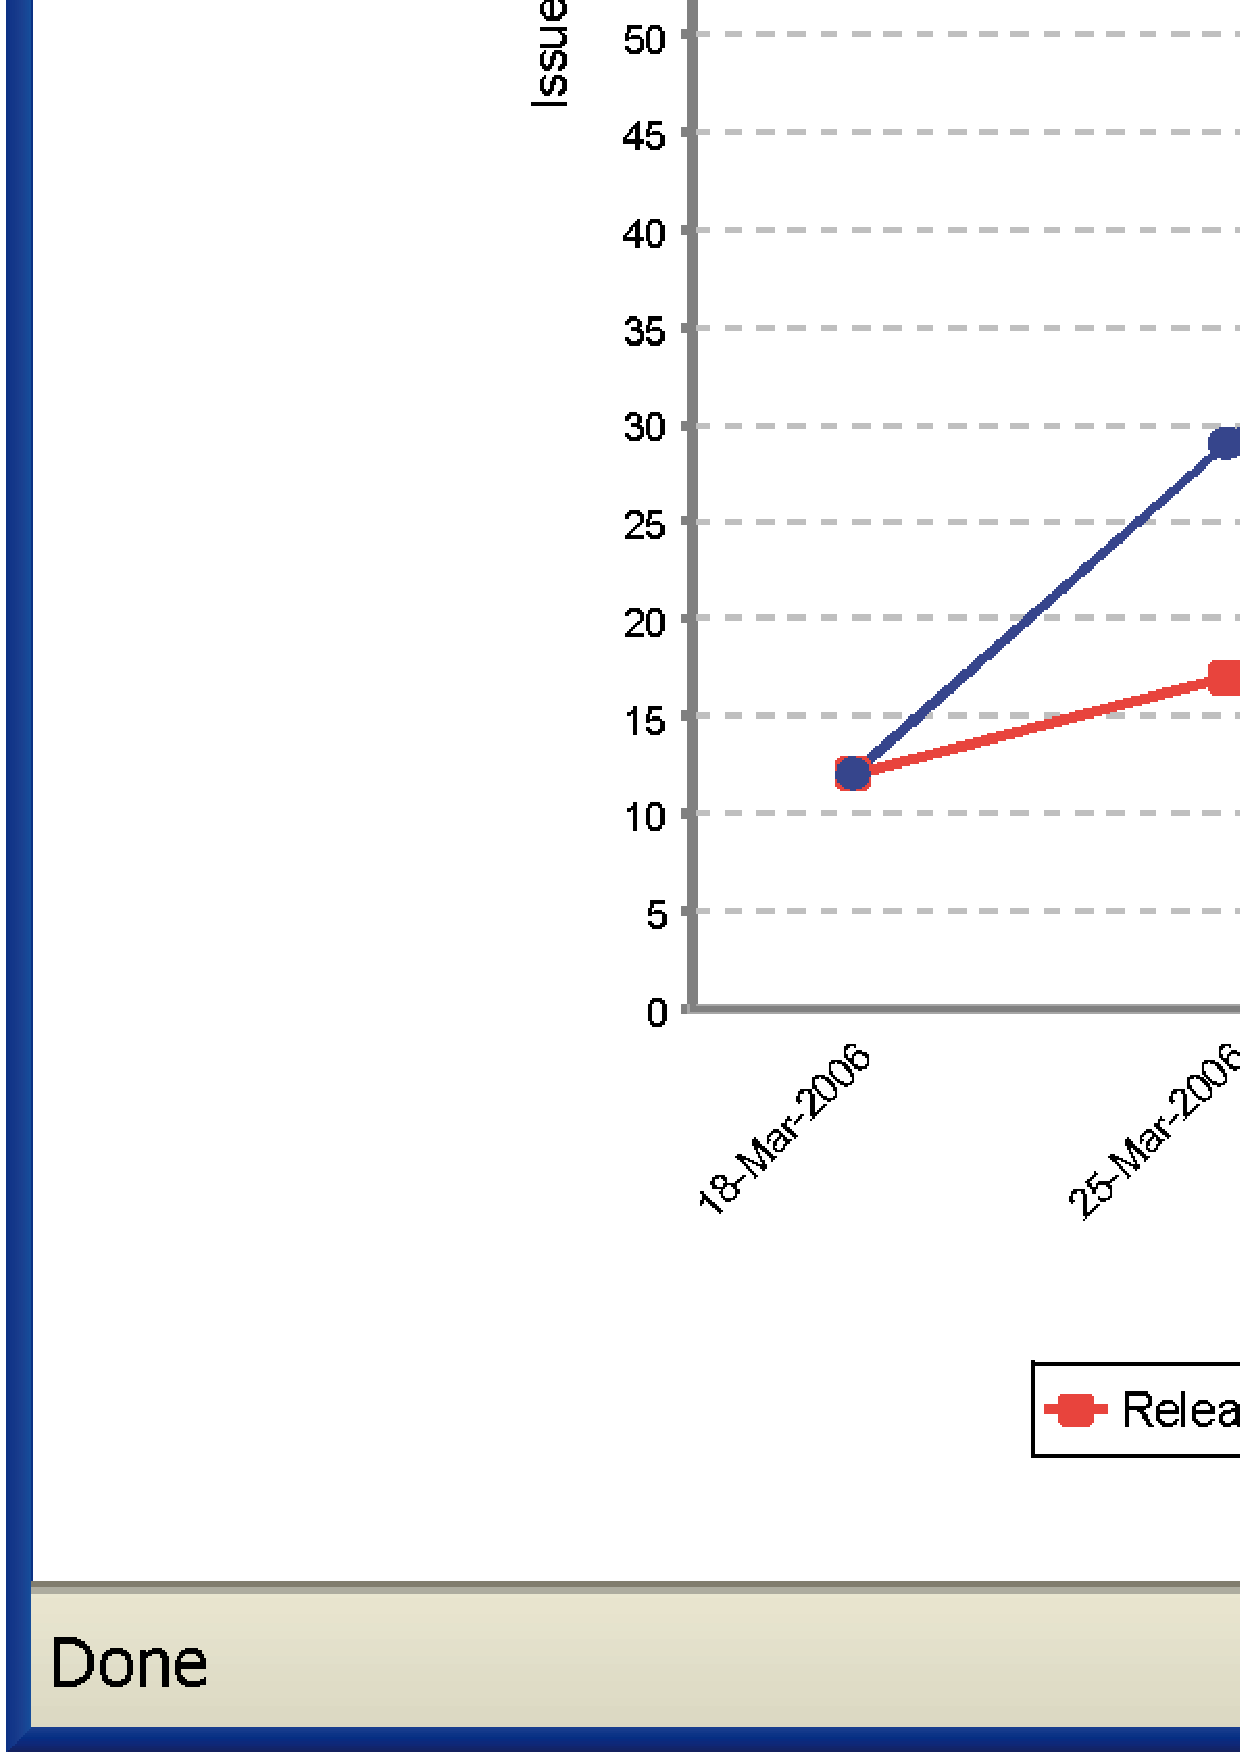
\includegraphics[height=0.90\textheight]{figures/ReleaseIssueTracking}
  \caption{Release Issue Tracking: Total vs. Open Issues} 
  \label{fig:ReleaseIssueTracking}
\end{figure}

An example of relatively high-level telemetry analysis is release cycle issue tracking. Figure \ref{fig:ReleaseIssueTracking} displays two issue tracking charts for ``Hackystat-7'' project release cycle 7.3 and 7.4 respectively. Each chart shows the total and remaining number of issues on the last day of each week during the two release cycles. The top blue line represents a telemetry stream for the total number of issues scheduled for that release; while the red line below represents a telemetry stream for the number of remaining issues. The release cycle is complete when the number of remaining issues touches zero. 
An interesting process level observation from the perspective of project management is that the manager did not schedule everything up-front. Instead, he added new issues almost every week. Nevertheless, he was able to manage the team to make consistent progress toward zero open issue to finish the release cycle. The red line (i.e., the bottom line) provided information about the trend in issue closure that helped the manager assess whether or not more issues could be added to that release cycle.
Another observation is that the telemetry charts in Figure \ref{fig:ReleaseIssueTracking} were generated when release cycle 7.4 was still in progress. By the end of May 6, 2006, there were still 11 open issues. From the perspective of project planning and scheduling, telemetry charts for previously finished release cycles, such as the chart on the top for release cycle 7.3, serve as the base line. By comparing the shape of telemetry streams in different release cycles, the project manager was able to make an in-process decision concerning whether the overall development process was stable, and estimate whether the team could finish the current release cycle on schedule.

Telemetry analysis can also be performed at a relatively low level to reveal details of software development process. An example of such an analysis is provided below, together with the introduction of basic telemetry language constructs: \textit{stream}, \textit{chart}, and \textit{report}. Figure \ref{fig:TelemetryReportChartStream} illustrates their relationship. 

\begin{figure}[p]
  \centering
  \includegraphics[height=0.90\textheight]{figures/TelemetryReportChartStream}
  \caption{Telemetry Report Analysis} 
  \label{fig:TelemetryReportChartStream}
\end{figure}

\clearpage
\subsubsection{Telemetry Report}

A telemetry report is a named set of telemetry charts that can be generated for a specified project over a specified time interval. The goal of a telemetry report is to discover how the trajectory of different process and product metrics might influence each other over time, and whether these influences change depending upon context.

For example, Figure \ref{fig:TelemetryReportChartStream} shows a telemetry report for ``Hacky2004-all'' project covering the time interval from the week of Feb 26, 2005 to the week of June 5, 2005. The report consists of two charts. Both charts show \textit{Unit Test Dynamics Telemetry}, which is an analysis of trends in the percentage of active time,\footnote{Active time is a proxy for developer effort and is based upon measuring the time spent writing and editing code inside an IDE.} allocated to testing (\textit{ActiveTime-Percentage}) the percentage of source code devoted to testing (\textit{JavaSLOC-Percentage}), and the percentage of test coverage that results from this effort and code (\textit{JavaCoverage-Percentage}). 

The two charts share the same time interval and project. The only difference is that they show unit test dynamics information for two different modules in the same project. Two developers are primarily responsible for the two modules respectively. Interestingly, the unit test dynamics telemetry trends for the two modules reveal a very different shape, indicating differences in the underlying approach to the development of the two modules. An important note is that software project telemetry does not presume any judgment as to which approach to development is better. Some projects might choose to trade a little testing for time-to-market. Others might require every single line of code perform exactly as intended.



\subsubsection{Telemetry Chart}

A telemetry chart is a named set of telemetry streams that can be generated for a specified project over a specified time interval. The goal of a telemetry chart is to display the trajectory over time of one or more process or product metrics.

For example, the same Figure \ref{fig:TelemetryReportChartStream} shows two instances of the same telemetry chart. Each chart contains three telemetry streams. You can see references to these three streams in the legend accompanying each chart. The legends also illustrate that telemetry streams can be parameterized: the top chart contains streams parameterized for the \textit{hackyZorro} module, while the bottom chart contains streams parameterized for the \textit{hackyCGQM} module.




\subsubsection{Telemetry Stream}

Telemetry streams are sequences of a single type of software process or product data for a single project over a specified time interval. They are best thought of as a kind of abstract data type representing one or more series of metric data values of the same type.

The time interval covered by a telemetry stream is divided into periods. The data points in each telemetry stream reflect the state of some key aspect of the software system under study during each period. The period can be relatively fine-grained such as \textit{daily}, or more coarse-grained such as \textit{weekly} or \textit{monthly}. Two types of information are typically represented by telemetry data points: 

\begin{itemize}
	\item Aggregated information --- The metrics values can be accumulated over the time period. Some examples are total coding effort, total lines added or deleted in the source code, total number of new bugs reported, etc.
	
	\item Snapshot information --- The metrics are only meaningful at a specific point in time. Some examples are the size of the source code, the number of open bugs, etc. Usually, the snapshot is taken at the beginning or at the end of each period.
\end{itemize}

For example, the time period used in the telemetry streams in Figure \ref{fig:TelemetryReportChartStream} is week. The data points in \textit{ActiveTime-Percentage} telemetry stream represent aggregated information. They are the total time spent on editing source code for the entire week. The data points in \textit{JavaSLOC-Percentage} and \textit{Coverage-Percentage} telemetry streams represent snapshot information. They are the number of source code lines and system test coverage at the end of each week. 

The advantage of telemetry is that it shows the history of some form of state in the project development environment, and helps the project manager detect changes in the development process. Another advantage is that it is generally tolerant of missing data. For example, there are missing dots in the telemetry streams in Figure \ref{fig:TelemetryReportChartStream}. While complete data provide the best support for project management or process improvement, occasional drop-outs of data should have little impact on the value of telemetry for decision-making. As a result, analyses built on top of telemetry streams can exhibit graceful degradation, providing value even when only partial data is available.




\subsubsection{Telemetry Language} \label{Intro:Solution:MetricsAnalysis:TelemetryLanguage}

Under the hood, telemetry reports, charts, and streams are generated using the telemetry language. The language serves two purposes:

\begin{itemize}
	\item Different software development environments and different projects might have different requirements for metrics analysis. The telemetry language provides a flexible mechanism that decouples the types of metrics we collect and the types of analyses we support.  
	\item Many interesting issues in software project management involve understanding the relationship between different metrics. For example, we might be interested in seeing whether an increased investment in code review pays off with less unit test failures, or increased test coverage, or less defects reported against the reviewed modules. The telemetry language enables interactive exploration of the relationship between metrics by allowing a user to experiment with the data to see what perspectives provides best insight into his/her particular situation.
\end{itemize}

The telemetry language that is used to generate the telemetry report in Figure \ref{fig:TelemetryReportChartStream} is listed below:


\begin{verbatim}
   streams ActiveTime-Percentage(filePattern1, filePattern2) = {
     "Active Time Percentage",
     
     ActiveTime(filePattern1, "false") 
     / ActiveTime(filePattern2, "false") 
     * 100
   };

   streams JavaCoverage-Percentage(filePattern) = {
     "Java Coverage Percentage",
     
     JavaCoverage("Percentage", filePattern, "method") 
   };
   
   streams JavaSLOC-Percentage(filePattern1, filePattern2) = {
     "Java SLOC Percentage",
     
     FileMetric("Java", "sourceLines", filePattern1)
     / FileMetric("Java", "sourceLines", filePattern2)
     * 100
   };

   y-axis yAxis(label) = {label};
   
   chart UnitTestDynamics-Chart(filePattern, testFilePattern) = {
     "Unit Test Dynamics Telemetry",
     
     (ActiveTime-Percentage(testFilePattern, filePattern), 
      yAxis("ActiveTime%")),
      
     (JavaCoverage-Percentage(filePattern), 
      yAxis("Coverage%")),
      
     (JavaSLOC-Percentage(testFilePattern, filePattern), 
      yAxis("SLOC%"))
   };

   report UnitTestDynamics-Hackystat-Report() = {
     "Unit Test Dynamics: Selected Hackystat Modules", 
     
     UnitTestDynamics-Chart("**/hackyZorro/**", 
                            "**/hackyZorro/**/Test*"),
     UnitTestDynamics-Chart("**/hackyCGQM/**", 
                            "**/hackyCGQM/**/Test*")
   };

   draw UnitTestDynamics-Hackystat-Report();
\end{verbatim}

Two features of the language are illustrated in the example above:
\begin{itemize}
	\item The telemetry language supports arithmetic operations. You can add, subtract, multiply, and divide two telemetry streams.
	
	\item The telemetry language supports parameterization. The two charts in the ``UnitTestDynamics-Hackystat-Report'' definition are the same except that they are passed two different parameter values representing two different modules in the project.
\end{itemize}


\begin{figure}[p]
  \centering
  
\includegraphics[height=0.90\textheight]{figures/TelemetryExpertAnalysis}
  \caption{Telemetry Expert Analysis} 
  \label{fig:TelemetryExpertAnalysis}
\end{figure}

Figure \ref{fig:TelemetryExpertAnalysis} shows the telemetry analysis expert interface. The telemetry charts generated are exactly the same as those in Figure \ref{fig:TelemetryReportChartStream}. The only difference is that this time we are using the telemetry language to interact with the system directly. Note, however, that the second chart is not shown in Figure \ref{fig:TelemetryExpertAnalysis} because of space constraint. The telemetry language specification in Appendix \ref{Chapter:TelemetryLanguageSpecification} contains more detailed information.







\subsection{Process Methodology}
\label{Intro:Solution:ProcessMethodology}


\begin{figure}[p]
  \centering
  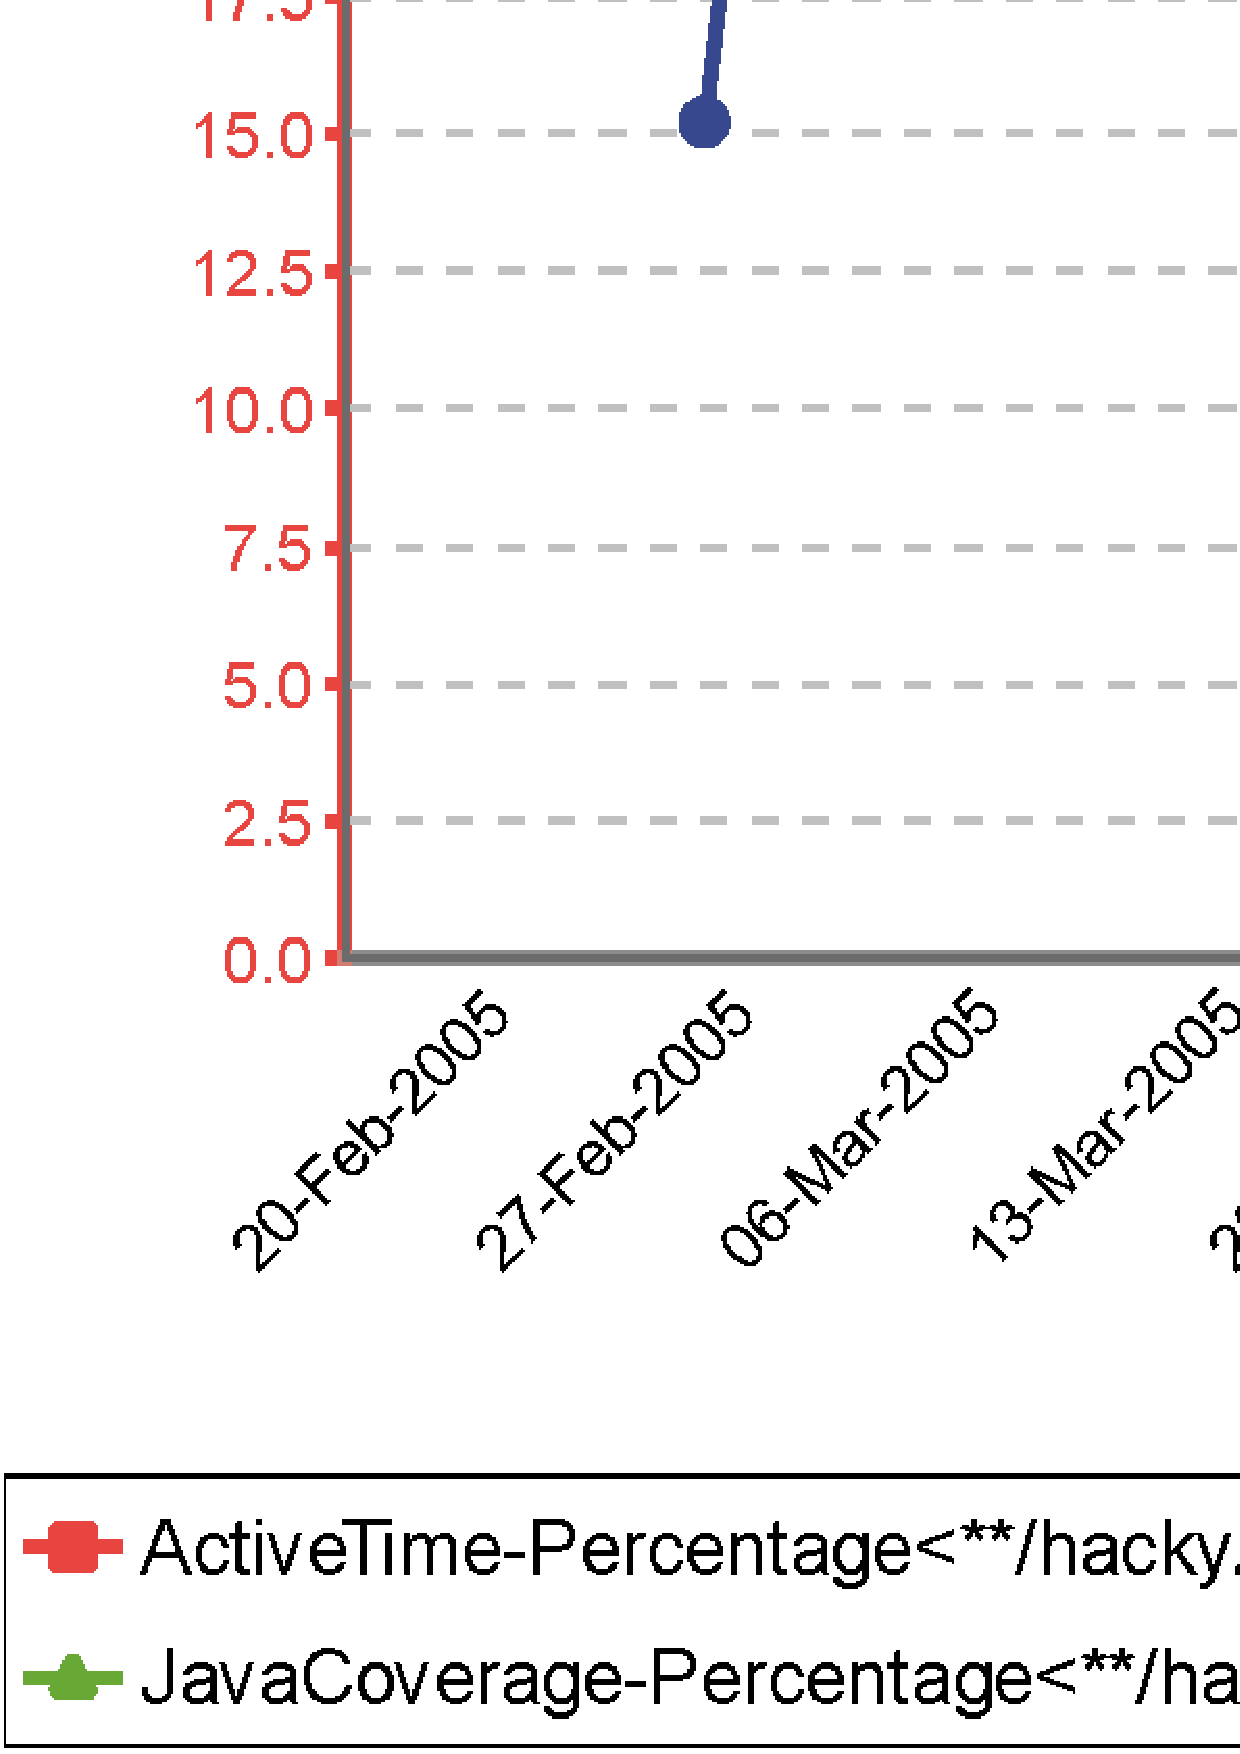
\includegraphics[width=1.00\textwidth]{figures/TelemetryChart}
  \caption{Telemetry Chart} 
  \label{fig:TelemetryChart}
\end{figure}

Figure \ref{fig:TelemetryChart} is an enlarged view of the top chart in Figure \ref{fig:TelemetryReportChartStream} and Figure \ref{fig:TelemetryExpertAnalysis}, showing unit test dynamics for the \textit{hackyZorro} module. 

A \textit{unit test} is a procedure used to verify that a particular module of source code is working correctly. This chart allows the comparison of the cost and the quality of unit testing. \textit{ActiveTime-Percentage} is the percentage of code-editing time allocated to writing test cases, and \textit{JavaSLOC-Percentage} is the percentage of source code lines that is unit test cases. Both of them are used as proxies for testing cost. \textit{JavaCoverage-Percentage} is the resulting test coverage (i.e., the percentage of the system exercised by test cases). It is used as a proxy for testing quality. Ideally, we wish to see high testing quality but low testing cost. When displayed in telemetry chart, we want to see the \textit{JavaCoverage-Percentage} telemetry stream near the top of the chart while the \textit{ActiveTime-Percentage} and \textit{JavaSLOC-Percentage} telemetry streams near the bottom of the chart. 

The telemetry chart in Figure \ref{fig:TelemetryChart} shows the development of the \textit{hackyZorro} module in the project. Both testing cost and testing quality were high at the beginning, but both were decreasing over time. After a little investigation, it turned out that the developer responsible for the module adopted \textit{test-driven development}\footnote{\textit{Test-driven development} is a programming technique emphasized in \textit{extreme programming} \cite{Beck:2000}. It requires writing test cases first before implementing the actual code.} methodology initially, but abandoned it during the development. This is very interesting. The telemetry streams in the chart clearly reveals the impact of the process-level changes\footnote{Again, the telemetry analysis does not presume any assumption that \textit{test-driven development} is better than other process methodologies. The judgment is left for the analysis user.}.

Telemetry streams consist of software process and product metrics. They are the basis of project management and process improvement. Telemetry charts and reports provide representation and display of telemetry trends. They make software developers more aware of their development processes by making them transparent and readily available. Telemetry streams for the same time interval are juxtaposed in the same telemetry chart or report to help developers detect covariance between different software metrics. For example, one might find that a drop in test coverage is frequently associated with an increase in the number of open bugs. This kind of information is important to project management, because it suggests a plausible causal relationship: low test coverage causes more bugs to slip through to the production stage. Based on this information, the project manager can implement changes to increase test coverage, and continue to use telemetry streams to monitor whether it indeed results in a decrease of the number of open bugs. At the same time, the project manager can monitor other telemetry streams, and check whether this corrective action has any unintended side effect to the development process. For example, he/she may wish to monitor productivity related telemetry streams to make sure that there is no reduction in developer productivity. The telemetry language provides a flexible mechanism decoupling the types of metrics and the types of analysis. It enables interactive exploration of the relationship between these different metrics. 

In general, applications of software project telemetry involve the following cycles to empirically guide the decision-making for project management and process improvement: 

\begin{enumerate}
  \item \textbf{Problem Detection} --- Use telemetry streams to monitor the development of a software project. Detect anomalies and undesirable trends in telemetry streams.
    
  \item \textbf{Process Improvement Hypothesis Generation} --- Determine plausible cause for the problem, and possible measure to correct it.
  
  \item \textbf{Process Change Implementation} --- Implement corrective measures.
  
  \item \textbf{Hypothesis Validation and Impact Analysis} --- Determine whether the problem goes away after corrective measures are implemented, and whether there are any unintended side effects caused by the corrective measures.

\end{enumerate}

The cycle continues until the project reaches completion.







%%%%%%%%%%%%%%%%%%%%%%%%%%%%%%%%%%%%%%%%%%%%%%%%%%%%%%%%%
%                                                       %
%                   S E C T I O N                       %
%                                                       %
%%%%%%%%%%%%%%%%%%%%%%%%%%%%%%%%%%%%%%%%%%%%%%%%%%%%%%%%%
\section{Thesis Statement}  \label{Intro:Thesis}

The claim of this thesis is that software project telemetry provides an effective approach to (1) automated metrics collection and analysis, and (2) in-process, empirically-guided software development process problem detection and diagnosis.

Compared to traditional model-base process prediction approaches, software project telemetry should be easier to use and cheaper to implement. It does not require software organizations to accumulate process and product metrics for finished projects in historical databases. Nor does it require expensive and error-prone model calibration before it can be used to make predictions. Instead, it focuses on evolutionary processes in development, and relies on metrics from an earlier stage of product development of the same project to make short-term predictions. For example, if system test coverage used to be almost 100\% but has been gradually dropping over time, then it may be a signal for management to re-allocate resources to improve project quality assurance. As a result, software project telemetry is best suited for in-process monitoring and control.

Software project telemetry should be robust. The information contained in telemetry streams should seldom be affected when there is occasional metrics drop out, and analyses should still provide decision-making value even if metrics collection starts midway through a project. 

Software project telemetry should also be flexible. There are no required set of metrics. Different software organizations can collect different sets of metrics according to their objectives, cost-benefit trade-offs, and measurement capabilities. For example, organizations with low process visibility can start with simple metrics such as source code size, and more metrics can be collected as their process matures and visibility increases.











%%%%%%%%%%%%%%%%%%%%%%%%%%%%%%%%%%%%%%%%%%%%%%%%%%%%%%%%%
%                                                       %
%                   S E C T I O N                       %
%                                                       %
%%%%%%%%%%%%%%%%%%%%%%%%%%%%%%%%%%%%%%%%%%%%%%%%%%%%%%%%%

\section{Empirical Evaluation}  \label{Intro:Evaluation}

The claim of this thesis was evaluated in two empirical studies: one in a classroom setting, and the other in the Collaborative Software Development Lab (CSDL). The primary goal was to assess metrics collection cost and decision-making value of software project telemetry. The secondary goal was to discover obstacles the developers might encounter during their use of the technology, and to gain insights about software project telemetry best practices and possible technology adoption barriers.
 
The classroom study was conducted in the two software engineering classes taught by Dr. Philip Johnson at the University of Hawaii in Spring 2005: one class for senior-level undergraduate students, and the other for introductory-level graduate students. By curriculum design, the students were divided into groups of 2 - 4 members collaborating on group projects and introduced to use software project telemetry to collect metrics and perform analyses on their own data. There were 25 students participating the study: 9 from the undergraduate session, and 16 from the graduate session.

The CSDL study was conducted in the Collaborative Software Development Lab at the University of Hawaii in Spring 2006, when a large scale software system (i.e., the Hackystat system itself) was being developed and maintained by a team of five on-site developers and a project manager. Three of the developers were Ph.D. students in software engineering (including me). They were hired by the lab working 20 hours a week. The other two were undergraduate students in their final semester. They were top students from the undergraduate software engineering class. They were working for the lab in exchange for personal development and course credit.

The two software development environments were quite different. In the classroom, there were a relatively large number of developers working on small scale class projects. In CSDL, there were a relatively small number of developers collaborating on a much larger project, which contained almost 300,000 lines of code and had been under development for five years. The CSDL developers had significantly more software engineering experience and process maturity compared to the average student in the classroom.

As a result, the two studies were structured differently. The classroom study was \textit{``passive''} in nature: though the students used software project telemetry to collect metrics and perform analyses on their own data, I did not make any deliberate attempts to help them improve their software development processes. On the other hand, the CSDL study was \textit{``active''} in nature: I introduced software project telemetry as a metrics-based process improvement program; I helped the project manager institute changes to improve project management practices; I also helped the developers gain insights into their development process.
Different data collection and analysis techniques were used in the two studies. 
The classroom study was relatively simple. My goal was to gather insights from a relatively large number of developers in a relatively short period of time. I distributed a questionnaire at the end of the semester to collect the student's opinions about software project telemetry. To increase my confidence in the validity of their self-reported opinions, I also analyzed their telemetry analysis invocation pattern to determine the extent to which their opinions were based on the actual system usage. 
In the CSDL study, I pursued a much more in-depth data collection and analysis strategy over a much longer period of time. I collected data from observations and interviews; I generated hypotheses from the data; I also tested the hypotheses in a limited way by making changes to the telemetry system or implementing new facilities to see whether the hypothesized outcome would come true or not.

The results of the two studies suggested that software project telemetry had acceptably-low metrics collection and analysis cost, and that it provided project management and process improvement decision-making values. 







%%%%%%%%%%%%%%%%%%%%%%%%%%%%%%%%%%%%%%%%%%%%%%%%%%%%%%%%%
%                                                       %
%                   S E C T I O N                       %
%                                                       %
%%%%%%%%%%%%%%%%%%%%%%%%%%%%%%%%%%%%%%%%%%%%%%%%%%%%%%%%%
\section{Contribution}  \label{Intro:Contribution}

There are three main contributions from this research:
\begin{enumerate}
	\item \textbf{The Concept of Software Project Telemetry}
	
In metrics collection, software project telemetry uses sensors to collect metrics automatically and unobtrusively. This sensor-based approach eliminates the chronic ``context-switch'' overhead inherent in manual approaches, such as PSP, and tool-assisted approaches, such as LEAP, PSP Studio, and Software Process Dashboard. 

In metrics decision-making, software project telemetry follows a light-weight approach by comparing telemetry trends in two different periods from the same project. The comparison involves a much smaller time scale than the whole project lifecycle. The metrics from the initial period of the project are used to establish a baseline and bootstrap the process. Project management and process improvement decisions are made by detecting changes in telemetry trends and comparing trends in two different periods in the same project. In-process control for a project that is still under development is made possible precisely because comparisons are made within a project. Since this approach does not involve the building of a statistical model in order to make cross-project comparison, it avoids many problems that typically exist in model-based approaches, such as spending the cost to accumulate a historical database of projects that may not be ``comparable'' to the current project. 

The two empirical studies I conducted showed that software project telemetry had sufficiently low metrics collection and analysis cost, and that it was able to deliver decision-making values, at least within the exploratory context of the two studies.

	
	\item \textbf{The Implementation of Software Project Telemetry}

Two pieces of software are the direct result of this thesis research. 
One of them is a server-side component, which includes the software code to interpret the telemetry language, the code to perform telemetry analyses and generate telemetry charts, and a web-based management console for telemetry construct definitions. The server-side component enables a user to log on to the server through a web browser to \textit{``actively''} explore relationships between different software metrics. 

The other is a client-side application that can be configured to automatically retrieve telemetry charts from the server and display them. It makes a sequence of telemetry charts continuously available to the user, providing \textit{``passive''} awareness of project status. 

The source code is GPL licensed, which encourages third-party improvement to be contributed back to the community. The system has already been adopted by several external sites, such as Sun Microsystem and the University of Maryland.

	
	\item \textbf{The Insights from the Empirical Studies}

Software project telemetry delivers best decision-making value when it can be customized to the specific needs of a software organization. The customization includes both setting up sensors to collect metrics and designing telemetry charts to perform analyses. ``Top-down telemetry design'' and ``bottom-up metrics collection'' are best practices. Top-down telemetry design refers to the idea that each telemetry chart should be designed with a clear purpose in mind, such as to help the development team meet a specific improvement goal. Bottom-up metrics collection refers to the recommendation to collect whatever metrics a software organization can. The rationale is the low cost associated with sensor-based metrics collection. Even if there is no apparent need for a metric today, it can still be used to establish a baseline for comparison tomorrow. 

Due to the automated nature of metrics collection in software project telemetry, broken sensors might not be noticed immediately. However, the empirical studies suggested that it would be possible to design special-purpose telemetry charts to help developers make quick assessments of whether the underlying sensors are sending data correctly or not. Therefore, another best practice for an organization is to deploy these special-purpose charts and assign a designated person to examine them.

One adoption barrier for this technology is concern about the level of privacy and confidentiality accorded to the data, especially with the effort-related personal process metrics. Though the current implementation has a mechanism to limit the kinds of data that could be accessed by people other than the owner, overcoming this issue seems largely dependent on what the data are used for in an organization. In other words, are the data used to improve development processes or to evaluate developers' performance? Lack of telemetry expertise within an organization might be another technology adoption barrier, since	software project telemetry will not likely deliver the best value if used straight ``out of the box'' and effective use, at least at this point, appears to require customization of the telemetry charts and reports.
	

\end{enumerate}







%%%%%%%%%%%%%%%%%%%%%%%%%%%%%%%%%%%%%%%%%%%%%%%%%%%%%%%%%
%                                                       %
%                   S E C T I O N                       %
%                                                       %
%%%%%%%%%%%%%%%%%%%%%%%%%%%%%%%%%%%%%%%%%%%%%%%%%%%%%%%%%
\section{Thesis Organization}  \label{Intro:Organization}

This thesis is organized into the following chapters:
\begin{itemize}
  \setlength{\itemsep}{0pt}
  \setlength{\parskip}{0pt}
  \item Chapter \ref{Chapter:Intro} is this chapter where the problem statement and proposed solution is described.
  
  \item Chapter \ref{Chapter:RelatedWork} relates the current research to the broader context of existing work.
  
  \item Chapter \ref{Chapter:Telemetry} describes software project telemetry in detail.
      
  \item Chapter \ref{Chapter:Implementation} describes the design details of an implementation of software project telemetry.

  \item Chapter \ref{Chapter:EvaluationStrategy} gives a brief review of research methods and discusses the evaluation strategies of software project telemetry.
  
  \item Chapter \ref{Chapter:EvaluationInClassroom} reports on a case study of software project telemetry in software engineering classes.
  
  \item Chapter \ref{Chapter:EvaluationInCSDL} reports on a case study of software project telemetry in the Collaborative Software Development Lab at University of Hawaii.

  \item Chapter \ref{Chapter:EvaluationConclusion} synthesizes the results from the two case studies to gain further insights.
  
  \item Chapter \ref{Chapter:Conclusion} provides final concluding remarks of this thesis research. 
\end{itemize}


